\documentclass[10pt]{article}
%$Id: macro.tex,v 1.10 2004/12/08 13:38:58 acary Exp $


%\usepackage{a4wide}
\textheight 25cm
\textwidth 16.5cm
\topmargin -1cm
%\evensidemargin 0cm
\oddsidemargin 0cm
\evensidemargin0cm
\usepackage{layout}


\usepackage{amsmath}
\usepackage{amssymb}
\usepackage{minitoc}
\usepackage{glosstex}
\usepackage{colortbl}
\usepackage{hhline}
\usepackage{longtable}

\usepackage{glosstex}
\def\glossaryname{Glossary of Notation}
\def\listacronymname{Acronyms}

\usepackage[outerbars]{changebar}\setcounter{changebargrey}{20}
\glxitemorderdefault{acr}{l}

%\usepackage{color}
\usepackage{graphicx,epsfig}
\graphicspath{{figure/}}
\usepackage[T1]{fontenc}
\usepackage{rotating}

%\usepackage{algorithmic}
%\usepackage{algorithm}
\usepackage{ntheorem}
\usepackage{natbib}


%\renewcommand{\baselinestretch}{2.0}
\setcounter{tocdepth}{2}     % Dans la table des matieres
\setcounter{secnumdepth}{3}  % Avec un numero.



\newtheorem{definition}{Definition}
\newtheorem{lemma}{Lemma}
\newtheorem{claim}{Claim}
\newtheorem{remark}{Remark}
\newtheorem{assumption}{Assumption}
\newtheorem{example}{Example}
\newtheorem{conjecture}{Conjecture}
\newtheorem{corollary}{Corollary}
\newtheorem{OP}{OP}
\newtheorem{problem}{Problem}
\newtheorem{theorem}{Theorem}


\newcommand{\CC}{\mbox{\rm $~\vrule height6.6pt width0.5pt depth0.25pt\!\!$C}}
\newcommand{\ZZ}{\mbox{\rm \lower0.3pt\hbox{$\angle\!\!\!$}Z}}
\newcommand{\RR}{\mbox{\rm $I\!\!R$}}
\newcommand{\NN}{\mbox{\rm $I\!\!N$}}

\newcommand{\Mnn}{\mathcal M^{n\times n}}
\newcommand{\Mnp}[2]{\ensuremath{\mathcal M^{#1\times #2}}}



\newcommand{\Frac}[2]{\displaystyle \frac{#1}{#2}}

\newcommand{\DP}[2]{\displaystyle \frac{\partial {#1}}{\partial {#2}}}

% c++ variables writting
\newcommand{\varcpp}[1]{\textit{#1}}
% itemize
\newcommand{\bei}{\begin{itemize}}
\newcommand{\ei}{\end{itemize}}

\newcommand{\ie}{i.e.}
\newcommand{\eg}{e.g.}
\newcommand{\cf}{c.f.}
\newcommand{\putidx}[1]{\index{#1}\textit{#1}}

\def\Er{{\rm I\! R}}
\def\En{{\rm I\! N}} 
\def\Ec{{\rm I\! C}}
 
\def\zc{\hat{z}}
\def\wc{\hat{w}}

\font\tete=cmr8 at 8 pt
\font\titre= cmr12 at 20 pt 
\font\titregras=cmbx12 at 20 pt

%----------------------------------------------------------------------
%                  Modification des subsubsections
%----------------------------------------------------------------------
\makeatletter
\renewcommand\thesubsubsection{\thesubsection.\@alph\c@subsubsection}
\makeatother

%----------------------------------------------------------------------
%             Redaction note environnement
%----------------------------------------------------------------------
\makeatletter
\theoremheaderfont{\scshape}
\theoremstyle{marginbreak}
\theorembodyfont{\upshape}
%\newtheorem{rque}{\bf Remarque}[chapter]
%\newtheorem{rque1}{\bf \fsc{Remarque}}[chapter] !!! \fsc est une commande french
\newtheorem{ndr1}{\textbf{\textsc{Redaction note}}}[section]

\newenvironment{ndr}%
{%
\tt
%\centerline{---oOo---}
\noindent\begin{ndr1}%
}%
{%
\begin{flushright}%
%\vspace{-1.5em}\ding{111}
\end{flushright}%
\end{ndr1}%
%\centerline{---oOo---}
}

\makeatother

%----------------------------------------------------------------------
%             Redaction note environnement V.ACARY
%----------------------------------------------------------------------
\makeatletter
\theoremheaderfont{\scshape}
\theoremstyle{marginbreak}
\theorembodyfont{\upshape}
%\newtheorem{rque}{\bf Remarque}[chapter]
%\newtheorem{rque1}{\bf \fsc{Remarque}}[chapter] !!! \fsc est une commande french
\newtheorem{ndr1va}{\textbf{\textsc{Redaction note V. ACARY}}}[section]

\newenvironment{ndrva}%
{%
\tt
%\centerline{---oOo---}
\noindent\begin{ndr1va}%
}%
{%
\begin{flushright}%
%\vspace{-1.5em}\ding{111}
\end{flushright}%
\end{ndr1va}%
%\centerline{---oOo---}
}

\makeatother
%----------------------------------------------------------------------
%             Redaction note environnement V.ACARY
%----------------------------------------------------------------------
\makeatletter
\theoremheaderfont{\scshape}
\theoremstyle{marginbreak}
\theorembodyfont{\upshape}
%\newtheorem{rque}{\bf Remarque}[chapter]
%\newtheorem{rque1}{\bf \fsc{Remarque}}[chapter] !!! \fsc est une commande french
\newtheorem{ndr1fp}{\textbf{\textsc{Redaction note F. PERIGNON}}}[section]

\newenvironment{ndrfp}%
{%
\tt
%\centerline{---oOo---}
\noindent\begin{ndr1fp}%
}%
{%
\begin{flushright}%
%\vspace{-1.5em}\ding{111}
\end{flushright}%
\end{ndr1fp}%
%\centerline{---oOo---}
}

\makeatother
%----------------------------------------------------------------------
%                  Chapter head enviroment
%----------------------------------------------------------------------
\newenvironment{chapter_head}
{%
\begin{center}%
-------------------- oOo --------------------\\%
\ \\%
\begin{minipage}[]{14cm}%
\noindent\normalsize\advance\baselineskip-1pt %
}%
{%
\par\end{minipage}%
\ \\%
\ \\%
-------------------- oOo --------------------
\end{center}%
\vspace*{\stretch{1}}%
\clearpage%
\thispagestyle{empty}%
\vspace*{\stretch{1}}%
\minitoc%
\vspace*{\stretch{2}}%
\clearpage%
}

%%% Local Variables: 
%%% mode: latex
%%% TeX-master: "report"
%%% End: 

\usepackage{psfrag}
\usepackage{fancyhdr}
\usepackage{subfigure}
%\renewcommand{\baselinestretch}{1.2}
\textheight 23cm
\textwidth 16cm
\topmargin 0cm
%\evensidemargin 0cm
\oddsidemargin 0cm
\evensidemargin 0cm
\usepackage{layout}
\usepackage{mathpple}
\makeatletter
\renewcommand\bibsection{\paragraph{References
     \@mkboth{\MakeUppercase{\bibname}}{\MakeUppercase{\bibname}}}}
\makeatother
%% style des entetes et des pieds de page
\fancyhf{} % nettoie le entetes et les pieds
\fancyhead[L]{Template 1 : Simulation of a two-dimensional bouncing ball -- V. Acary }
%\fancyhead[C]{V. Acary}%
\fancyhead[R]{\thepage}
%\fancyfoot[L]{\resizebox{!}{0.7cm}{\includegraphics[clip]{logoesm2.eps}}}%
\fancyfoot[C]{}%
%\fancyfoot[C]{}%
%\fancyfoot[R]{\resizebox{!}{0.7cm}{\includegraphics[clip]{logo_cnrs_amoi.ps}}}%
%\addtolength{\textheight}{2cm}
%\addtolength{\textwidth}{2cm}
%\pagestyle{empty}
%\renewcommand{\baselinestretch}{2.0}
\begin{document}
%\layout
\thispagestyle{empty}
\title{WP2 Template 1 \\
 Simulation of a bouncing ball with \\ the Moreau's Time--Stepping scheme}
\author{V. Acary}

\date{Version 1.0 \\
 \today}
\maketitle


\pagestyle{fancy}

\section{Description of the physical problem : A bouncing ball on a plane}
\label{Sec:description}


Let us consider  a ball of  mass $m$ and radius $R$, described by $3$ generalized coordinates $q=(z,x,\theta)$. The ball is subjected to the gravity $g$ and a vertical external force $f(t)$. The system is also constituted by a rigid plane, defined by its position $h$ with respect to the axis $Oz$. We assume that the position of the plane is fixed. The physical problem  is depicted on the Figure~\ref{Fig:2D-BouncingBall}. 




\begin{figure}[htbp]
  \centering
  \psfrag{O}{$\mathsf{O}$}
  \psfrag{z}{$\mathsf{z}$}
  \psfrag{x}{$\mathsf{x}$}
  \psfrag{h}{$\mathsf{h}$}
  \psfrag{g}{$\mathsf{g}$}
  \psfrag{theta}{${\theta}$}
  \psfrag{R}{${\mathsf R}$}
  \psfrag{f}{${\mathsf{f(t)} }$}
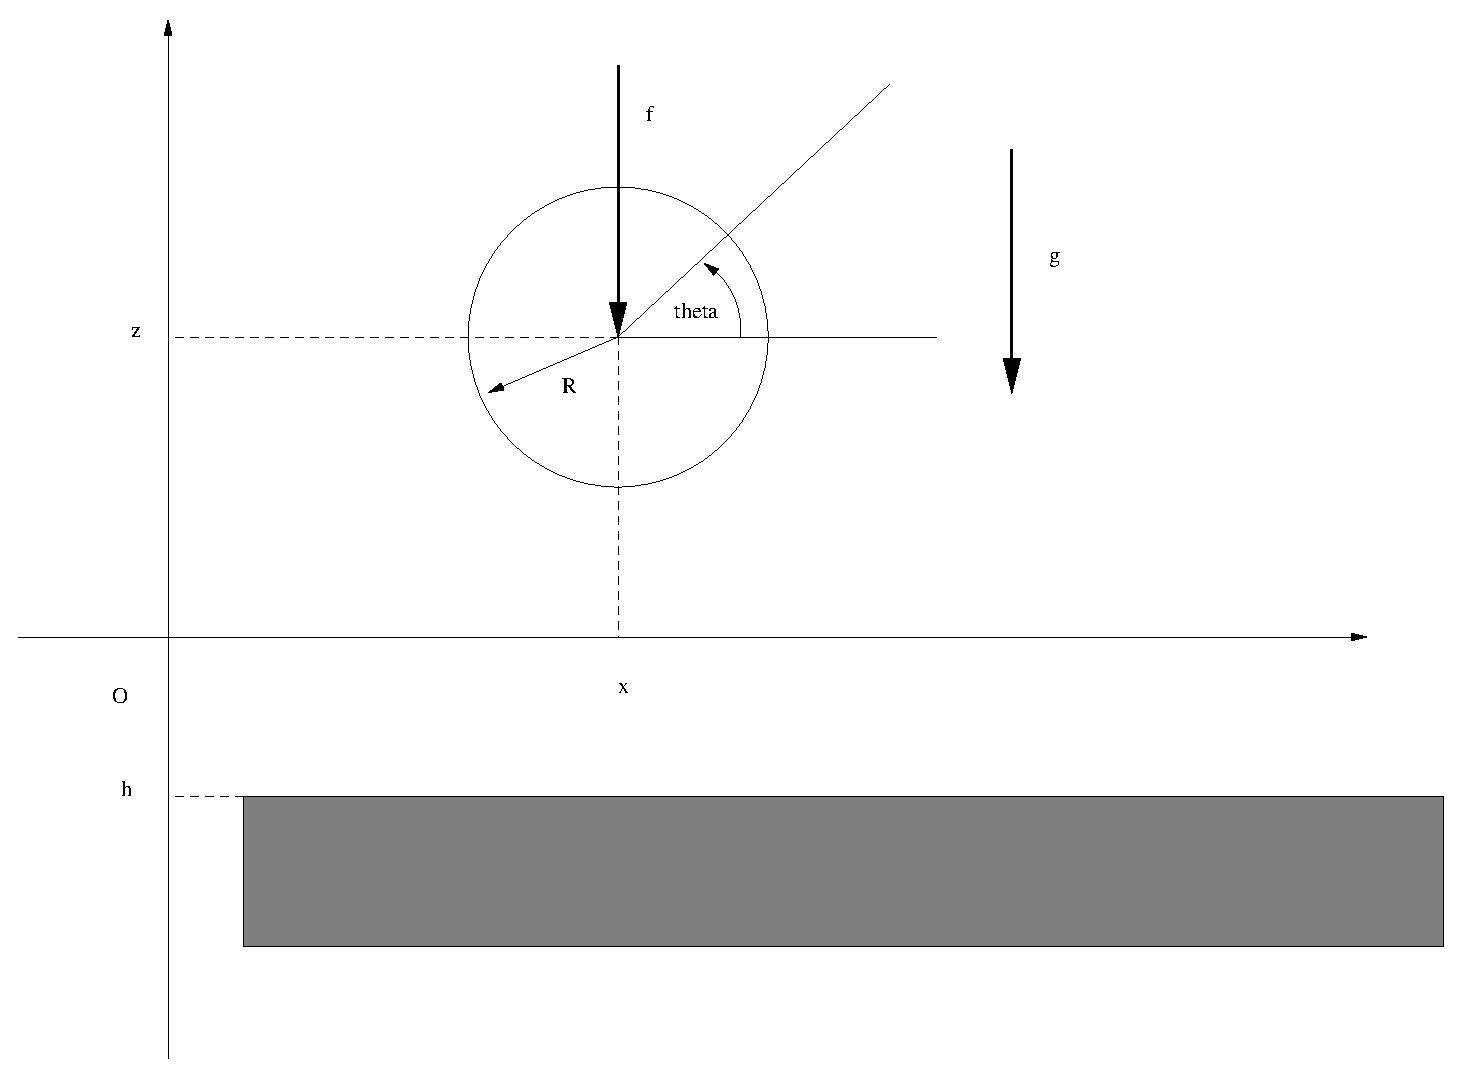
\includegraphics[width=0.6\textwidth]{./2D-BouncingBall.eps}
  \caption{Two-dimensional bouncing ball on a rigid plane}
  \label{Fig:2D-BouncingBall}
\end{figure}

The ball bounces on the rigid plane, introducing a constraint on the position of the ball. We consider also that the behavior of the system at impact is governed by a Newton impact law with a coefficient of restitution $e$.

%% \begin{ndr}
%%   Do we need to be more precisely on the specific format for rigid bodies ?
%% \end{ndr}







\section{Definition of a general abstract class of NSDS: The Lagrangian NSDS}
\label{Sec:descriptionNSDS}



In this section, we provide a short description of a general abstract class of Non Smooth Dynamical system (NSDS): The Lagrangian NSDS. More generally, we will try to present this type of system in a more general framework where the NSDS consists of:
\begin{enumerate}
\item a dynamical system with boundary conditions in terms of state variables,
\item a set of input/output variables and theirs relations with the state variables,
\item a set of  nonsmooth laws which rely  the input/output variable.
\end{enumerate}


%% \begin{ndrva}
%%   Is a Lagrangian NSDS actually constituted by the complete set : Dynamical equation + relation + non smooth laws  or just by the dynamical equation + relation ? 

%% Indeed, it seems that the Non Smooth Law is a very generic object which can be independently defined. Just dynamical equation + relation, are application dependent and may constitute the class of Lagrangian dynamical system with specific output.
%% \end{ndrva}

\subsection{Dynamical system and Boundary conditions}


\paragraph{General non linear case.} The equation of evolution of a Lagrangian system may be stated as follows :
\begin{eqnarray}
  \label{eq:1}
  M(q)\ddot q + Q(q,\dot q) + F(\dot q, q , t) = F_{ext}(t) + r
\end{eqnarray}
where 
\begin{itemize}
\item $q \in \RR^n$ is the generalized coordinates vector. The dimension $n$  of this vector is called  the number of degree of freedom of the system. The first and the second time derivative of $q$, denoted $\dot q$ and $\ddot q$, are usually called the velocity and the acceleration of the system.
\item $M(q): \RR^n \mapsto \mathcal M^{n\times n}$ is the inertia term 
\item $Q(q,\dot q ): \RR^n \times \RR^n \mapsto \mathcal \RR^{n}$ is the non linear inertia term,
\item $F(\dot q, q , t) : \RR^n \times \RR^n \times \RR \mapsto \mathcal \RR^{n}$ is the internal force of the system,
\item $F_{ext}(t):  \RR \mapsto \mathcal \RR^{n}  $  is the given external force,
\item $r \in \RR^n$ is the force due the nonsmooth law.
\end{itemize}


In a general way, we denote the state of the system as 
\begin{eqnarray}
  x =  \left[\begin{array}{c}
  q \\
  \dot q
  \end{array}\right] 
\end{eqnarray}
which is a vector of dimension $2\times n$.  The equation of evolution \eqref{eq:1} may be reformulated in terms of the state vector as :
\begin{equation}
  \label{eq:2}
\dot x =f (x,t) +  \left[\begin{array}{c}
  0 \\
  I
  \end{array}\right] r
\end{equation}
which is a classical order one formulation for an ordinary differential equation (ODE).

\begin{remark}
In most mechanical applications, the order one form is not very convenient for the  numerical applications.  Furthermore the specific structure of the Lagrangian system allow us to use of special numerical algorithms to solve it. 
\end{remark}

\paragraph{A particular case: the linear time invariant case.}

In this case, all of the operators defined above are linear time invariant. In this case, we can define it directly provided that the following matrices are given :
\begin{itemize}
\item $M\in \mathcal M^{n\times n}  $ is the mass matrix
\item $F(\dot q, q , t) = C \dot q + K q  $ where $ C \in \mathcal M^{n\times n}  $ is the viscosity matrix and $K \in \mathcal M^{n\times n}$   is the stiffness matrix.
\end{itemize}
\paragraph{Boundary conditions}
The boundary conditions are given for an Initial Value Problem (IVP) as :
\begin{equation}
  \label{eq:3}
  t_0 \in \RR,\quad q(t_0)=q_0 \in \RR^{n}, \quad \dot q(t_0)=\dot q_0\in \RR^{n},
\end{equation}and for a Boundary Value Problem (BVP) :
\begin{equation}
  \label{eq:4}
   (t_0,T) \in \RR\times \RR , \quad \Gamma(q(t_0),\dot q(t_0),q(T),\dot q(T))=0
\end{equation}



\subsection{Relation between constrained variables and state variables}


\paragraph{Formal Case.} In a general way, the dynamical system is completed by a set of non smooth laws which do not  concern  directly the state vector. The set of such variables, denoted $y$, on which we apply the constraints, depends, in a very general way, of the state vector $x$, the time $t$ and possibly the force $r$ :
\begin{eqnarray}
  \label{eq:y}
  y=h(x,r,t).
\end{eqnarray}

In the same way, we have to specify the relation between $r$, the force due to the constraints, and $\lambda$ associated to $y$ through the nonsmooth law:
\begin{equation}
  \label{eq:5}
  r=g(x, \lambda,t).
\end{equation}

\paragraph{Linear time invariant case} In the linear time invariant case, this relation are directly given by matrices defined by :
\begin{eqnarray}
  \label{eq:6}
  y&=& C x + D \lambda, \\ 
  r&=& B \lambda.
\end{eqnarray}
 
\paragraph{Lagrangian system}
In the Lagrangian systems, the structure of theses relations is very particular  and we assume that they can be written as :
\begin{eqnarray}
  \label{eq:7}
   y&=& h(q),\\
   \dot y &=& H(q)^{T}\dot q, \\
   r &=& H(q) \lambda.
\end{eqnarray}

We can also consider the linear case such as 
\begin{eqnarray}
  \label{eq:8}
      y &=& H^{T} q + b,\\
      \dot y &=& H^{T}\dot q, \\
      r &=& H \lambda,
\end{eqnarray}
which can be stated by assumptions or derived by a linearization procedure of \eqref{eq:7}.

In order to give more meaning to this choice, let us recall the definition of a constraint (or a joint) in a  mechanical system :
\begin{eqnarray}
  \label{eq:9}
  y=h(x,t) = h(q,\dot q,t)  &=&0 \text{ in the bilateral case,}\\
 &\geq& 0 \text{ in the unilateral case. } 
\end{eqnarray}

 If we assume that these relations are non holonomic i.e., independence with respect to the velocity $\dot q$, we are used to derive for perfect constraint  the relative velocity as:
\begin{equation}
  \label{eq:10}
  \dot y= \nabla^T_q h(q,t) \dot q + \DP{h(q,t)}{t}.
\end{equation}
Furthermore, if the constraints is scleronomic ( i.e., independence with respect to the time  $t$) this relation leads to 
\begin{eqnarray}
  \label{eq:11}
   \dot y= \nabla^T_q h(q) \dot q.
\end{eqnarray}

Indeed, the gradient corresponds $\nabla^T_q h(q)$ to the normal to the constraints that we denoted $\boldsymbol n$. A first part of the more general mapping $H(q)$ is the given by the normal $\boldsymbol n$, which corresponds to a basis transportation. The rest of the mapping $H(q)$ is given by the tangential part.

The independence of the power with the respect of various frames and the notion of  a perfect constraint require that the relation between $\lambda$ and $r$ is given  by :
\begin{eqnarray}
r =  \nabla_q h(q) \lambda
\end{eqnarray}




%% \begin{ndr}
%%   We can see that the definition of such relations are very dependent of the application. The definition of rather general relations as above are not very convenient. This remark leads to the fact that such relation are part of the complete Lagrangian model. In LMGC, such relations define the behavior between a body and a contactor.
%% \end{ndr}



\subsection{Definition of the Non Smooth Law between constrained variables}

Several kind of nonsmooth laws may be formulated for a  Lagrangian system. For the purpose of this template, we define just the unilateral contact law and the impact law.

The unilateral contact law may formulated as follows :
\begin{eqnarray}
  \label{eq:12}
  0 \leq y \perp r\geq 0
\end{eqnarray}
and the Newton impact law :
\begin{eqnarray}
  \label{eq:13}
  \text{if } y(t)=0,\quad  \dot y(t^+)= -e   \dot y(t^-)
\end{eqnarray}

 
\section{The Formalization of the bouncing ball problem into the class of Lagrangian NSDS}
We assume that the system of a bouncing ball on a plane belongs to the abstract class of the Lagrangian NSDS. 

\subsection{Dynamical equation}

 From the input of the physical data, we construct all of the terms which defined a Lagrangian NSDS.   In our special case, the model is completly linear:
\begin{eqnarray}
  q&=&       \left[\begin{array}{c}
  z \\
  x \\
  \theta
  \end{array}\right]    \\
  M(q)&=&
  \left[\begin{array}{ccc}
  m &0 &0 \\
  0 & m & 0 \\
  0 & 0 & I
  \end{array}\right] \text{ where } I=\Frac 3 5 m R^2 \\
  Q(q,\dot q )& = &\left[\begin{array}{c}
  0 \\
  0  \\
  0
  \end{array}\right]  \\
  F(q, \dot q , t) &=&  \left[\begin{array}{c}
  0 \\
  0  \\
  0
  \end{array}\right] \\
  F_{ext}(t)& = & \left[\begin{array}{c}
  -m g \\
  0  \\
  0
  \end{array}\right] +  \left[\begin{array}{c}
  f(t)\\
  0  \\
  0
  \end{array}\right]
\end{eqnarray}

\subsection{relations}

The unilateral constraint requires that :
\begin{eqnarray}
  \label{eq:14}
  z-R -h \geq 0
\end{eqnarray}
so we identify the terms of the equation~(\ref{eq:8}) 
\begin{eqnarray}
  \label{eq:15}
  y&=&H^{T}q+b\\
  H^{T}&=& \left[
  \begin{array}[]{ccc}
  1 & 0 & 0
  \end{array}\right] \\
  b &=& -R - h
\end{eqnarray}

In the same way, the reaction due to the constraint is written as follows : 
\begin{eqnarray}
  \label{eq:16}
  r  = H \lambda, \text{ with } H = \left[
  \begin{array}[]{c}
  1 \\ 0 \\ 0
  \end{array}\right] 
\end{eqnarray}
\subsection{Non Smooth laws}

In the case of the bouncing ball, there is just one unilateral constraint such that :
\begin{eqnarray}
  \label{eq:17}
  0 \leq y \perp \lambda\geq 0
\end{eqnarray}

 The Newton impact law at impact is given by  :
\begin{eqnarray}
  \label{eq:18}
  \text{if } y=0,\quad  \dot y(t^+)= -e   \dot y(t^-)
\end{eqnarray}




\section{Description of the numerical strategy: the Moreau's Time--stepping scheme}
\label{Sec:Simulation}



\subsection{Time discretization of the dynamical system}

We provide in this section a time discretization method of the Lagrange dynmical system (\ref{eq:1}), consistent with the non smooth character of the solution. Let us consider here only the linear time invariant case. The equation  may be reformulated equivalently in terms of an integral over a time step $[t_i,t_{i+1}]$ of length $h$ such that :
\begin{eqnarray}
  \int_{[t_i,t_{i+1}]} M \ddot q + C \dot q + K q \,dt =  \int_{[t_i,t_{i+1}]} F_{ext}(t)\,dt +  \int_{[t_i,t_{i+1}]} r \,d\nu
\end{eqnarray}

Due to the non smooth character of the motion, the first term is integrated by an one order scheme( backward Euler-like) such that :
\begin{eqnarray}
  \label{eq:19}
   \int_{[t_i,t_{i+1}]} M \ddot q  \, dt \approx M (\dot q(t_{i+1})-\dot q(t_{i})) 
\end{eqnarray}

For simplicity sake, we note the approximation of $q$ and $\dot q$:
   \begin{eqnarray}
     \label{eq:20}
     \dot q_{i+1}\approx\dot q(t_{i+1}),  \dot q_{i}\approx \dot q(t_{i})
   \end{eqnarray}

 For the other terms, a $\theta$-method is used :
 \begin{eqnarray}
\int_{[t_i,t_{i+1}]}  C \dot q + K q \,dt &\approx& h\left[\theta  (C \dot q_{i+1}+K q_{i+1}) + (1-\theta) (C \dot q_{i}+K q_{i})  \right]\\
 \int_{[t_i,t_{i+1}]} F_{ext}(t) \,dt &\approx& h\left[\theta  F_{ext}(t_{i+1})+(1-\theta)  F_{ext}(t_{i})  \right]\\
 \end{eqnarray}

For the term which contains the reaction force, we state a new variable such as :
\begin{eqnarray}
  \label{eq:21}
  R_{i+1} = \frac  1 h \int_{[t_i,t_{i+1}]} r \,d\nu
\end{eqnarray}

The displacement is integrated through the velocity with :
\begin{eqnarray}
  \label{eq:22}
  q_{i+1} = q_{i} +  h\left[\theta  \dot q_{i+1}+(1-\theta)  \dot q_{i}  \right]\\
\end{eqnarray}

Finally, we obtain the time discretized equation of motion as follows :
\begin{eqnarray}
  \label{eq:23}
  \left[M+h\theta C + h^2 \theta^2 K\right] (\dot q_{i+1} - \dot q_{i}) = - h  C \dot q_{i} - h K q_{i} - h^2 \theta  K \dot q_{i}
+  h\left[\theta  F_{ext}(t_{i+1})+(1-\theta)  F_{ext}(t_{i})  \right]  +h R_{i+1},
\end{eqnarray}
which can be written :
\begin{eqnarray}
  \label{eq:24}
   \dot q_{i+1} = \dot q_{free}  + h W R_{i+1}
\end{eqnarray}
where 
\begin{eqnarray}
  W &=&   \left[M+h\theta C + h^2 \theta^2 K\right]^{-1}\\
 \dot q_{free} &=& \dot q_{i}+  W \left[   - h  C \dot q_{i} - h K q_{i} - h^2 \theta  K \dot q_{i}
+  h\left[\theta  F_{ext}(t_{i+1})+(1-\theta)  F_{ext}(t_{i})  \right]       \right]
\end{eqnarray}

The free velocity $ \dot q_{free}  $ correponds to the velocity of the system without any constraints.

\subsection{Time discretization of the relations}
The Time discretization of the relations is fully implicit and may be written as :
\begin{eqnarray}
  \label{eq:25}
      y_{i+1} &=& H^{T} q_{i+1} + b\\
      \dot y_{i+1} &=& H^{T}\dot q_{i+1} \\
      R_{i+1} &=& H \lambda_{i+1}
\end{eqnarray}

\subsection{Time discretization of the Non Smooth laws}



A natural way of discretizing the unilateral constraint  leads to the following implicit discretization :
\begin{eqnarray}
  \label{eq:26}
  0 \leq y_{i+1} \perp  \lambda_{i+1}  \geq 0
\end{eqnarray}

In the Moreau's time--stepping, we use a reformulation of the unilateral constraints in terms of velocity \eqref{eq:26} :
\begin{eqnarray}
  \label{eq:27}
   \text{If } y(t) =0, \text{ then } 0 \leq \dot y \perp  \lambda  \geq 0
\end{eqnarray}
which leads to the following discretisation :
\begin{eqnarray}
  \label{eq:28}
   \text{If } y^{p} \leq 0, \text{ then } 0 \leq \dot y_{i+1} \perp  \lambda_{i+1}  \geq 0
\end{eqnarray}
 where $y^{p}$ is a prediction of the position at time $t_{i+1}$, for instance,    $y^{p} = y_{i} + \Frac{h}{2}  \dot y_i$.

If we want to introduce now the Newton impact law, we consider an equivalent velocity defined by
\begin{eqnarray}
  \label{eq:29}
  \dot y^{e}_{i+1} = \dot y_{i+1} + e \dot y_{i}
\end{eqnarray}
and we apply the constraints directly on this velocity :
\begin{eqnarray}
  \label{eq:30}
  \text{If } y^{p} \leq 0, \text{ then } 0 \leq \dot y^{e}_{i+1} \perp  \lambda_{i+1}  \geq 0
\end{eqnarray}


\subsection{Summary of the time discretized equations}
\begin{eqnarray}
  \dot q_{i+1} &=& \dot q_{free}  + h W R_{i+1} \\
  q_{i+1} &=& q_{i} +  h\left[\theta  \dot q_{i+1}+(1-\theta)  \dot q_{i}  \right] \\
  \dot y_{i+1} &=& H^{T}\dot q_{i+1} \\
  R_{i+1} &=& H \lambda_{i+1}\\
  y^{p} &=& y_{i} + \Frac{h}{2}  \dot y_i\\
  \text{If }&y^{p}& \leq 0, \text{ then } 0 \leq \dot y^{e}_{i+1} \perp  \lambda_{i+1}  \geq 0
\end{eqnarray}

This set of equations can be reduced to a ``condensed'' system in terms of $\dot y^{e}_{i+1}$ and ${\lambda_{i+1}}$ :
\begin{eqnarray}
  \dot y^{e}_{i+1} &=&  H^{T} \dot q_{free} + h H^{T} W H \lambda_{i+1}  + e \dot y_{i}\\
  y^{p} &=& y_{i} + \Frac{h}{2}  \dot y_i\\
  \text{If }&y^{p}& \leq 0, \text{ then } 0 \leq \dot y^{e}_{i+1} \perp  \lambda_{i+1}  \geq 0
\end{eqnarray}



\subsection{Numerical Strategy}

The numerical stratgey is given by the pseudo-algorithm \ref{Algo:MTS}.

\begin{algorithm}
  \begin{algorithmic}
{
    \REQUIRE Classical form of the synamical equation : $ M, K, C, F_{ext}, q_0, \dot q_0$
    \REQUIRE  Classical form of the relations : $ H, b$
    \REQUIRE  Classical form of the non smooth law  : $ e$
    \REQUIRE Numerical parameter : $ h, \theta, T, t_0$
    \ENSURE  $(\{ q_n\}, \{ \dot q_n\},\{R_n\}) $     
    \STATE // Construction of time independant operators :
    \STATE $ W = \left[M+h\theta C + h^2 \theta^2 K\right]^{-1}$ // The iteration matrix 
    \STATE $ w = H^{T} W H $ // The LCP matrix (Delassus operator)
    \STATE // Time discretization $n_{step} := [ \frac{T-t_0}{h}]$
    \STATE // Non Smooth Dynamical system integration
    \FOR{$i=0$ to $n_{step}$ }
        \STATE // Computation of $\dot q_{free}$
        \STATE $\dot q_{free} = \dot q_{i}+  W \left[   - h  C \dot q_{i} - h K q_{i} - h^2 \theta  K \dot q_{i}
+  h\left[\theta  F_{ext}(t_{i+1})+(1-\theta)  F_{ext}(t_{i})  \right]       \right]$
        \STATE // Prediction of the constrained variables
        \STATE $q^{p} = q_i + \frac h 2 \dot q_i\,; \qquad y^{p} = H^T q^p +b $
        \STATE // Contact detection
        \IF{$y^{p} \leq 0$} 
        \STATE // Formalization of the one-step  LCP
        \STATE $ bLCP =  H^{T} \dot q_{free}  + e \dot y_{i}$
        \STATE // Resolution  of the one-step LCP
        \STATE $ [\dot y^{e}_{i+1}, \lambda_{i+1}]=$\texttt{solveLCP}$(w,bLCP)$
        \ENDIF
        \STATE // State Actualisation
        \STATE $R_{i+1} = H \lambda_{i+1} $
        \STATE $\dot q_{i+1} = \dot q_{free}  + h W R_{i+1}$
        \STATE $q_{i+1} = q_{i} +  h\left[\theta  \dot q_{i+1}+(1-\theta)  \dot q_{i}  \right]$
     \ENDFOR}
  \end{algorithmic}
  \caption{Moreau's Time Stepping scheme}
\label{Algo:MTS}
\end{algorithm}

%\clearpage



\section{Exploitation of the results}
\label{Sec:Results}

For the case of Lagrangian NSDS, the state variable and the reaction force vs. time are the basic results that we want to export out of the algorithm. Various of energies may be also expected by the user. 


\begin{figure}[htbp]
 \subfigure[Position of the ball vs. Time]{  \includegraphics[angle=-90,width=0.49\textwidth]{position.eps}}
 \subfigure[Velocity of the ball vs. Time]{ \includegraphics[angle=-90,width=0.49\textwidth]{velocity.eps}}
 \subfigure[Reaction due to the contact force vs. Time]{\includegraphics[angle=-90,width=0.5\textwidth]{Impulse.eps}}
 \subfigure[Energy balance vs.time]{\includegraphics[angle=-90,width=0.5\textwidth]{energy.eps}}
  \caption{Results}
  \label{Fig:PositionVelocity}
\end{figure}


\section{First analysis for the architectural point of view}
\label{Sec:Analysis}

To be defined \ldots

\end{document}
